\documentclass[9pt]{beamer}
% \documentclass[notes, handout, 9pt]{beamer}
% \documentclass[handout, 9pt]{beamer}

\usepackage{import}
\subimport{../}{preamble.tex}
\subimport{../}{beamer-theme.tex}

% Location for all figures / pictures
\graphicspath{{pictures/}{figures/}}

\usepackage{tikz}
\usetikzlibrary{calc}
\usepackage{pgfplots}


%--------------------------------------------------
% Presentation Information
%--------------------------------------------------
\title[Continuous Optimization]{Black-Box Optimization Methods}
\author[]{\textbf{Bart Van Parys}}
\date[]{Fall 2026}
%--------------------------------------------------

\begin{document}

\begin{frame}  

  \maketitle

  \vspace{-2em}
  
    \begin{center}
    \begin{tabular}{lll}
      Instructor : & \textbf{Bart Van Parys} & \textbf{(\href{mailto:mastermath@vanparys.xyz}{mastermath@vanparys.xyz})} \\
    \end{tabular}
  \end{center}
  
\end{frame}

\section{Performance of Numerical Methods}

\begin{frame}{A Problem Instance}

  An optimization \emph{problem instance} is
  \[
    \begin{array}{rl}
      p^\star = \min & f(x) \\[0.5em]
      \st & x\in X \\[0.5em]
      & g(x) \geq b \\
    \end{array}
  \]
  for a particular cost function $f$, constraint function $g$, and budgets $b$.

  \vfill

  \uncover<2->{
    \emph{Fastest algorithm:} Output always $(p^\star, x^\star)$.
  } 

  \vfill

  \uncover<3->{
  It does not make sense to discuss algorithmic performance based on a single problem instance.
  }
\end{frame}

\begin{frame}{The Black Box Model}

  A black-box optimization problem consists of
  \begin{itemize}
  \item \emph{Class} $\Sigma$: Collection of instances
  \item \emph{Oracle} $\mc O$: Oracle information about instance of interest
  \item \emph{Accuracy} $\mc T_\epsilon$ : Stopping criteria
  \end{itemize}

  \vfill

  \uncover<2->{
    \textbf{Example:}
    \begin{center}
      \begin{tabular}{r|l}
        \hline
        Optimization Problem & Example \\[0.5em]
        \hline
        Class $\Sigma$ & $\min_{x\in[0, 1]^n} f(x)$ \\[0.5em]
                             & $f$ is $L$-Lipschitz\\
        Oracle $\mc O$ & zero-order oracle $x\mapsto f(x)$.\\[0.5em]
        Accuracy $\mc T_\epsilon$ & Find $\bar x$ such that $f(\bar x)-f(x^\star)\leq\epsilon$.\\[0.5em]
        \hline
      \end{tabular}
    \end{center}
  }
\end{frame}

\begin{frame}{General Iterative Method}

  \begin{algorithm}[H]
    \SetKwInput{Initialization}{Initialization}
    \Initialization{Starting point $x_0$; Accuracy $\epsilon>0$.\\ Counter $k=0$; Information $I_{-1}=\emptyset$.}
    \While{Accuracy $\mc T(x_k)>\epsilon$}{
      Call oracle $\mc O$ at $x_k$.\\
      Update the information set: $I_k = I_{k-1}\cup (x_k, \mc O(x_k))$.\\
      Apply rules of method $M$ to $I_k$ and form $x_{k+1}$.
    }
    \Return $x_k$
    \caption{General Iterative Scheme}
  \end{algorithm}

\end{frame}


\begin{frame}{Complexity}

  \begin{itemize}
    \setlength\itemsep{2em}
  \item \textbf{Analytical Complexity}: The \emph{worst-case} number of \emph{oracle calls} to solve any instance $\mc P$.
  \item<2-> \textbf{Algorithmic Complexity}: The \emph{worst-case} number of \emph{elementary operations} to solve any instance $\mc P$.
  \end{itemize}
  
\end{frame}

\begin{frame}{Optimization Algorithms}

  When going about designing optimization algorithms \emph{two roads} can be taken.

  \vfill
  
  \begin{enumerate}
    \setlength\itemsep{2em}
  \item Universal optimization algorithm capable of solving all problems \\[1em]

  \item<2-> Many optimization algorithms, each of which dedicated to a very particular class of problems
    \begin{itemize}
      \setlength\itemsep{1em}
    \item Linear optimization problems
    \item Quadratic optimization problems
    \item Convex optimization problems
    \item Integer optimization problems
    \item \dots
    \end{itemize}
  \end{enumerate}

  \vspace{1em}

  \uncover<3->{
  \textbf{Let us see where the first path takes us.}
  }
\end{frame}

\section{Optimization Problems are Hard}

\begin{frame}{Lipschitz continuity}

  Let $f:[0, 1]^n\to\Re$ be a Lipschitz continuous function, i.e.,
  \[
    \forall x, y\in [0, 1]^n : \quad \abs{f(x)-f(y)}\leq \red{L} \norm{x-y}.
  \]
  The \emph{Lipschitz constant} $\red{L}$ measures how ill-defined the optimization problem is.

  \vfill

  \begin{center}
    \includegraphics[height=4.5cm]{lipschitz/lipschitz.pdf}
  \end{center}
  
\end{frame}

\begin{frame}{Universal Optimization Problem}

  \emph{Lipschitz Optimization Problem :} Let $f:[0, 1]^n\to\Re$ be a Lipschitz continuous function, i.e.,
  \[
    \forall x, y\in [0, 1]^n : \quad \abs{f(x)-f(y)}\leq \red{L} \norm{x-y}_{\emph{\infty}}.
  \]
  Find a point $\hat x \in [0, 1]^n$ such that $f(\hat x) - f^\star \leq \red{\epsilon}$ where
  \[
    \begin{array}{rl}
      f^\star \defn \inf  & f(x) \\[1em]
                    \st  & x \in [0, 1]^n.
    \end{array}
  \]

  \vfill

  \uncover<2->{
    \begin{center}
    \begin{tabular}{r|l}
      \hline
      Optimization Problem & Example \\[0.5em]
      \hline
      Model $\Sigma$ & $\min_{x\in[0, 1]^n} f(x)$ \\[0.5em]
      & $f$ is $L$-Lipschitz\\
      Oracle $\mc O$ & zero-order oracle $x\mapsto f(x)$.\\[0.5em]
      Accuracy $\mc T_\epsilon$ & Find $\hat x$ such that $f(\hat x)-f(x^\star)\leq\epsilon$.\\[0.5em]
      \hline
    \end{tabular}
  \end{center}
  }
\end{frame}

\begin{frame}{Gridding Method}
  
  \textbf{Grid Method :} evaluate the function $f$ on each point
  \[
    x = \left(\frac{i_1}{p}, \dots, \frac{i_n}{p}\right),
  \]
  where $0\leq i_1, \dots, i_n\leq p$ and take for $\hat x$ the one that minimizes $f$.

  \vfill
  
  \textbf{Complexity : } $(p+1)^n$ evaluations of $f$.

  \vfill

  Commonly used optimization method.

\end{frame}

\begin{frame}{Gridding Method : Accuracy}

  \textbf{Theorem} ({Gridding accuracy}):
  \[
    f(\hat x) - f^\star \leq \frac{L}{2 p}
  \]

  \textbf{Proof :} Let $\bar x$ be the grid point closest to the optimal solution $x^\star$. Evidently, we have that $\norm{\bar x-x^\star}_\infty\leq 1/(2p)$. We have that
  \[
    f(\bar x) - f^\star = \abs{f(\bar x) -f(x^\star)} \leq L \norm{\bar x - x^\star}_\infty \leq L/(2p),
  \]
  from the Lipschitz continuity of $f$.

  \vfill

  \begin{center}
    \includegraphics[height=2.5cm]{gridding/gridding.pdf}
  \end{center}
 
\end{frame}


\begin{frame}{Gridding Method : Accuracy}

  \textbf{Theorem} ({Gridding accuracy}):
  \[
    f(\hat x) - f^\star \leq \frac{L}{2 p}
  \]

  \vfill

  \textbf{Corollary :} The grid method needs \emph{at most} $$\left(\ceil{\frac{L}{2\epsilon}}+1\right)^n$$
    function evaluations to find $\hat x$ such that $f(\hat x) - f^\star \leq \epsilon$.
 
\end{frame}



\begin{frame}{Best Universal Method}

  \textbf{Theorem : } Any optimization algorithm with $\epsilon < L/4$ for the class of Lipschitz continuous functions on $[0, 1]^n$ requires \emph{at least} $(\floor{\frac{L}{2\epsilon}}-1)^n$ evaluations of $f$.

  \vfill
  
  The proof is based on the concept of a ``resisting oracle'' or worst-case function. Interpretation as a game against an adversary.
  
\end{frame}

\begin{frame}{Resisting Oracle}

  \begin{center}
    \uncover<2->{
    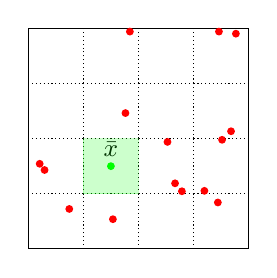
\begin{tikzpicture}[scale=0.7]
      % \foreach \x in {0,1,...,4}
      % {
      %   \foreach \y in {0,1,...,4}
      %   {
      %     \node[circle,inner sep=1,fill=black] at (\x, \y) {};
      %   }
      %   }

      \pgfmathsetseed{1}


      % Feasible set
      \draw (0, 0) -- (0, 4) {};
      \draw (0, 0) -- (4, 0) {};
      \draw (4, 4) -- (0, 4) {};
      \draw (4, 4) -- (4, 0) {};

      
      \foreach \x in {0,1,...,3}
      {
        \foreach \y in {0,1,...,3}
        {
          \only<3->{
          \draw[densely dotted] (\x, \y) -- (\x+1, \y) {};
          \draw[densely dotted] (\x, \y) -- (\x, \y+1) {};
          }
        }
      }

      
      \foreach \x in {4}
      {
        \foreach \y in {0,1,...,3}
        {
          \only<3->{
            \draw[densely dotted] (\x, \y) -- (\x, \y+1) {};
          }
        }
      }

      \foreach \x in {0,1,...,3}
      {
        \foreach \y in {4}
        {
          \draw[densely dotted] (\x, \y) -- (\x+1, \y) {};
        }
      }


      \foreach \p in {1, ...,  15}
      {        
        \node[circle,inner sep=1,fill=red] at (4*rnd, 4*rnd) {};        
      }
      
      \uncover<4->{
      \node[circle,inner sep=1,fill=green] (xbar) at (1.5, 1.5) {};
      \node[above] at (xbar) {\small $\bar x$};
      \draw[draw=green, fill=green, opacity=0.2] (1,1) rectangle (2,2);
      }

      % \node[circle,inner sep=1,fill=red] (xstar) at (1.75, 1.65) {};
      % \node[right, red] at (xstar) {\small $x^\star$};
    \end{tikzpicture}
    }
  \end{center}

  \begin{itemize}
  \item Notice that $p \defn \floor{\frac{L}{2\epsilon}}-1$ and $\epsilon<L/4$ implies $1\leq p<\frac{L}{2\epsilon}$ and $\epsilon<\frac{L}{2p}$. 
  \item<2-> Suppose method evaluates $f$ on merely $p^n-1$ points for which resisting oracle always returns $0$. Hence, $\min_{k} f(x_k)=0$.
  \item<3-> Consider a grid with spacing $1/p$. There must be a grid cell without a point $x_k$ in the interior. Let $\bar x$ be its center.
  \item<4-> Recall that $\norm{\bar x -x_k}_\infty\geq \frac{1}{2 p}$ for any $x_k$. The function
    \[
      f^{\rm{oracle}} = x\mapsto \min(0, L (\norm{x-\bar x}_\infty-\tfrac{1}{(2 p)}))
    \]
    is $L$-Lipschitz and consistent with the function evaluations, i.e., $f^{\rm{oracle}}(x_k)=0$.
  \item<5-> However, $f^{\rm{oracle}}(\bar x) = -\tfrac{L}{(2p)}< -\epsilon$; a contradiction. 
  \end{itemize}
  
\end{frame}

\begin{frame}{The gridding method in perspective}

  Lipschitz optimization has \textbf{complexity} at least $$\left(\floor{\frac{L}{2\epsilon}}-1\right)^n$$ function evaluations.
  
  \vfill
  
  Take $n=16$, $\epsilon=0.01$ and $L=1$, best universal optimization method needs at least
  \[
    1,104,427,674,243,920,646,305,299,201
  \]
  evaluations.

  \vfill

  \begin{itemize}
  \item Heuristics can be tried (genetic algorithms, ant optimization, \dots) \emph{without guarantees}.
  \end{itemize}
  
\end{frame}

\begin{frame}{Optimization Algorithms}

  When going about designing optimization algorithms two roads can be taken.

  \vfill
  
  \begin{enumerate}
    \setlength\itemsep{2em}
  \item Universal optimization algorithm capable of solving all problems \\[1em]
  \item Many optimization algorithms, each of which dedicated to a very particular class of problems
    \begin{itemize}
      \setlength\itemsep{1em}
    \item Linear optimization problems
    \item Quadratic optimization problems
    \item Convex optimization problems
    \item Integer optimization problems
    \item \dots
    \end{itemize}
  \end{enumerate}

  \vfill

  \emph{We are only left with the second road.}
  
\end{frame}

\begin{frame}{Focus on specific class of problems}

  \begin{center}
    \begin{tcolorbox}[width=6cm]
      \begin{equation}
        \tag{$\mc P$}
        \begin{array}{rl}
          \minimize & f(x) \\[1em]
          \st & x \in Q
        \end{array}
      \end{equation}
    \end{tcolorbox}
  \end{center}
  \vfill

  Theoretically efficient optimization methods:
  \begin{itemize}
    \setlength\itemsep{2em}
  \item should be applied to a specific problem class.
    \begin{itemize}
      \setlength\itemsep{1em}
    \item Linear optimization
    \item Convex optimization
    \item Differentiable optimization
    \item \dots
    \end{itemize}
  \item Are characterized by the way it extracts information on the specific instance of the problem.
  \end{itemize}
  
\end{frame}

\section{Convex Optimization}

\begin{frame}{Black-Box Convex Model}

  \begin{minipage}{0.4\textwidth}
    \begin{equation}
      \label{opt:problem}
      \tag{$\mc P$}
      \begin{array}{rl}
        \minimize & f(x) \\[1em]
        \st & x \in Q
      \end{array}
    \end{equation}
  \end{minipage}%
  \hfill
  \begin{minipage}{0.55\textwidth}
    \begin{itemize}
    \item $Q$ is a convex set
    \item $f:\Re^n\to\Re$ is a convex function
    \item $\epsilon$ is desired accuracy
    \end{itemize}
  \end{minipage}

  \vfill
  
  \begin{center}
    \begin{tabular}{r|l}
      \hline
      Optimization Problem & Convex Optimization Problem \\[0.5em]
      \hline
      Model $\Sigma$ & $\min_{x\in Q} f(x)$ \\[0.5em]
      & $f$ and $Q\subseteq \Re^n$ are convex \\[0.5em]
      Oracle $\mc O$ & first-order oracle $x\mapsto \partial f(x)$.\\[0.5em]
      Accuracy $\mc T_\epsilon$ & Find $\hat x$ such that $f(\hat x)-f(x^\star)\leq\epsilon$.\\[0.5em]
      \hline
    \end{tabular}
  \end{center}
  
\end{frame}

\begin{frame}{The Bisection Method}

  \begin{minipage}{0.4\textwidth}
    \begin{equation*}
      \begin{array}{rl}
        \minimize & f(x) \\[1em]
        \st & x \in [a, b]
      \end{array}
    \end{equation*}
  \end{minipage}%
  \hfill
  \begin{minipage}{0.55\textwidth}
    \begin{itemize}
    \item $f:\Re\to\Re$ is a convex function
    \item $\max \set{f(x)-f(y)}{x, y\in [a, b]} \leq V$
    \item oracle : $x\mapsto (f(x), g(x))$ with $g(x) \in \partial f(x)$
    \item $\epsilon$ is desired absolute accuracy
    \end{itemize}
  \end{minipage}

  \vfill
  
  \textbf{The bisection method :}

  \vfill
  
  \begin{minipage}{0.3\textwidth}
    \centering
    \includegraphics[height=3.25cm]{bisection/bisection-1.pdf}
  \end{minipage}%
  \hfill
  \begin{minipage}{0.3\textwidth}
    \centering
    \includegraphics[height=3.25cm]{bisection/bisection-2.pdf}
  \end{minipage}%
  \hfill
  \begin{minipage}{0.3\textwidth}
    \centering
    \includegraphics[height=3.25cm]{bisection/bisection-3.pdf}
  \end{minipage}
  

\end{frame}

\begin{frame}{The Bisection Method}

  \begin{minipage}{0.4\textwidth}
    \begin{equation*}
      \begin{array}{rl}
        \minimize & f(x) \\[1em]
        \st & x \in [a, b]
      \end{array}
    \end{equation*}
  \end{minipage}%
  \hfill
  \begin{minipage}{0.55\textwidth}
    \begin{itemize}
    \item $f:\Re\to\Re$ is a convex function
    \item $\max \set{f(x)-f(y)}{x, y\in [a, b]} \leq V$
    \item oracle : $x\mapsto (f(x), g(x))$ with $g(x) \in \partial f(x)$
    \item $\epsilon$ is desired absolute accuracy
    \end{itemize}
  \end{minipage}

  \vfill
  
  \begin{algorithm}[H]
    \SetKwInput{Initialization}{Initialisation}
    \Initialization{$\ell_0\defn a$, $u_0\defn b$, $d_0\defn 1$, $k\defn 0$}
    \While{$d_k\geq\epsilon/V$}{
      $x_k \defn (u_k+\ell_k)/2$, $d_{k+1}\defn d_k/2$\;
      \lIf{$g(x_k)>0$}{
        $\ell_{k+1}\defn \ell_k, u_{k+1}\defn x_k$
      }
      \lIf{$g(x_k)<0$}{
        $\ell_{k+1}\defn x_k, u_{k+1}\defn u_k$
      }
      \lIf{$g(x_k)=0$}{
        $d_{k+1}\defn 0$
      }
    }
    \Return best $x_k$ seen
    \caption{Bisection}
  \end{algorithm}

  \vfill

  \textbf{Complexity : } at most $\ceil{ \log_2(V/\epsilon)}$ calls to oracle.

\end{frame}

\begin{frame}{Proof [$\star$]}

  \begin{itemize}

  \item Let $x^\star \in [\ell_N, u_N]$ after $N\geq \log_2(V/\epsilon)$ iterations
  \item By construction we have that
    \[
      f(y) \geq f(\hat x) = \min_{k\in [1, \dots, N]} f(x_k) \quad \forall y \not\in [\ell_N, u_N]
    \]
  \item Define $Q^\alpha \defn \set{(1-\alpha) x^\star+\alpha y}{y\in Q=[a,b]}\subseteq Q$ for some $\alpha\in (2^{-N}, 1]$.
  \item Evidently, $Q^\alpha$ has length $\alpha (b-a)$, while $[\ell_N, u_N]$ has length $2^{-N} (b-a)$. There must exist a point $$z=(1-\alpha) x^\star+\alpha y$$ with
    $y\in [a, b]$ and $z\in Q^\alpha$ but $z\not\in [\ell_N, u_N]$.
  \item From convexity we have
    \[
      f(z) \leq (1-\alpha) f(x^\star) + \alpha f(y) \implies f(z) - f(x^\star) \leq \alpha (f(y)-f(x^\star)) \leq \alpha V.
    \]
  \item We have $z\not\in [\ell_N, u_N] \implies f(\hat x) \leq f(z)$ and hence $f(\hat x)-f(x^\star)\leq \alpha V$ for any $\alpha \in (2^{-N}, 1]$. We conclude that
    $f(\hat x)-f(x^\star)\leq \inf_{\alpha\in (2^{-N}, 1]}\alpha V = 2^{-N}V \leq \epsilon$.
  \end{itemize}
  
\end{frame}

\begin{frame}{The Bisection Method}

  \textbf{Theorem :} Finding an $\epsilon$-solution to $\min_{x\in [-1, 1]}\, f(x)$, where $\max \set{f(x)-f(y) }{x, y\in [-1, 1]} \leq 1$ takes
  \[
    \ceil {\frac 13 \log_2(\tfrac 1\epsilon)} \leq N \leq \ceil{\log_2(\tfrac 1\epsilon)} ~~\rm{queries}
  \]
  
\end{frame}

\begin{frame}{The Bisection Method}

  \begin{center}
    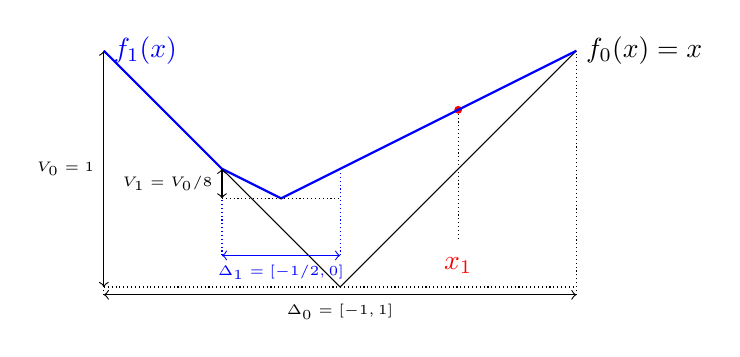
\begin{tikzpicture}

      % The funciton $f_i$
      \draw[black] (-3,3) -- (0,0) -- (3,3);
      \node[right] at (3,3) {$f_0(x)=\abs{x}$};

      \draw[densely dotted] (-3, 0) -- (3, 0);
      \draw[<->, black] (-3,-0) -- (-3,3);
      \node[left] at (-3, 1.5) {\tiny $V_0=1$};
      
      % The set $\Delta_i$
      \draw[<->, black] (-3,-0.1) -- (3,-0.1);
      \node[below] at (0, -0.1) {\tiny $\Delta_0=[-1, 1]$};
      \draw[densely dotted] (-3, -0.1) -- (-3, 3);
      \draw[densely dotted] (3, -0.1) -- (3, 3);


      \uncover<2->{
      \node (x0) at (1.5, 0.5) {};
      \node[below, red] at (x0) {$x_1$} {};
      \draw[densely dotted] (1.5, 2.25)  -- (x0) ;
      }
      

      \uncover<3->{
        \node[circle, inner sep=1, fill=red] (f0) at (1.5, 2.25) {};
      % The funciton $f_{i+1}$
      \draw[blue, thick] (-3,3) -- (-1.5,1.5) -- (-0.75,1.125) -- (0, 1.5) -- (3,3);

      % The set $\Delta_{i+1}$
      \draw[<->, blue] (-1.5, 0.4) -- (0, 0.4);
      \node[below, blue] at (-0.75, 0.4) {\tiny $\Delta_{1}=[-1/2, 0]$};
      \draw[blue, densely dotted] (-1.5, 0.4) -- (-1.5, 1.5);
      \draw[blue, densely dotted] (0, 0.4) -- (0, 1.5);

      \node[blue, right] at (-3,3) {$f_{1}(x)$};
    }

    \uncover<4->{
    \draw[densely dotted] (-1.5, 1.125) -- (0, 1.125);
    \draw[<->, black] (-1.5,1.125) -- (-1.5,1.5);
    \node[left] at (-1.5, 1.3125) {\tiny $V_1=V_0/8$};
    }
    \end{tikzpicture}
  \end{center}

  \textbf{Resisting Oracle:}
  \begin{itemize}
  \item Initialize $f_0=\abs{x}$ with $\Delta_0=[-1,1]$ and $V_0=1$.
  \item<2-> Suppose algorithm evaluates oracle at $x_1\geq 0$. (Other case is symmetric.)
  \item<3-> Construct a new function $f_1$ which outside of $\Delta_0$ equals $f_0$. Return $f_1(x_1)$.
  \item<4-> Function $f_1$ has minimum in $\Delta_1=[-1/2, 0]$ where the oracle has never been called.
  \item<5-> If $x_2\not\in \Delta_1$; Set $f_2(x)=f_1(x)$ and return $f_2(x)$.
  \item<6-> If $x_2\in \Delta_1$; Apply previous procedure locally to $\Delta_1$.
  \end{itemize}
  
\end{frame}

\begin{frame}{The Bisection Method}

  \begin{center}
    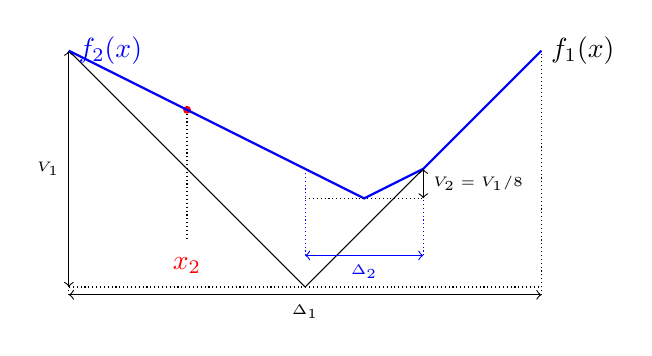
\begin{tikzpicture}

      % The funciton $f_i$
      \draw[black] (-3,3) -- (0,0) -- (3,3);
      \node[right] at (3,3) {$f_1(x)$};

      \draw[densely dotted] (-3, 0) -- (3, 0);
      \draw[<->, black] (-3,-0) -- (-3,3);
      \node[left] at (-3, 1.5) {\tiny $V_1$};
      
      % The set $\Delta_i$
      \draw[<->, black] (-3,-0.1) -- (3,-0.1);
      \node[below] at (0, -0.1) {\tiny $\Delta_1$};
      \draw[densely dotted] (-3, -0.1) -- (-3, 3);
      \draw[densely dotted] (3, -0.1) -- (3, 3);


      \uncover<2->{
      \node (x0) at (-1.5, 0.5) {};
      \node[below, red] at (x0) {$x_2$} {};
      \draw[densely dotted] (-1.5, 2.25)  -- (x0) ;
      }
      

      \uncover<3->{
        \node[circle, inner sep=1, fill=red] (f0) at (-1.5, 2.25) {};
      % The funciton $f_{i+1}$
      \draw[blue, thick] (-3,3) -- (0,1.5) -- (0.75,1.125) -- (1.5, 1.5) -- (3,3);

      % The set $\Delta_{i+1}$
      \draw[<->, blue] (0, 0.4) -- (1.5, 0.4);
      \node[below, blue] at (0.75, 0.4) {\tiny $\Delta_{2}$};
      \draw[blue, densely dotted] (0, 0.4) -- (0, 1.5);
      \draw[blue, densely dotted] (1.5, 0.4) -- (1.5, 1.5);

      \node[blue, right] at (-3,3) {$f_{2}(x)$};
    }

    \uncover<4->{
    \draw[densely dotted] (0, 1.125) -- (1.5, 1.125);
    \draw[<->, black] (1.5,1.125) -- (1.5,1.5);
    \node[right] at (1.5, 1.3125) {\tiny $V_2=V_1 /8$};
    }
    \end{tikzpicture}
  \end{center}

  \textbf{Resisting Oracle:}
  \begin{itemize}
  \item Initialize $f_0=\abs{x}$ with $\Delta_0=[-1,1]$ and $V_0=1$.
  \item Suppose algorithm evaluates oracle at $x_1\geq 0$. (Other case is symmetric.)
  \item Construct a new function $f_1$ which outside of $\Delta_0$ equals $f_0$. Return $f_1(x_1)$.
  \item Function $f_1$ has minimum in $\Delta_1=[-1/2, 0]$ where the oracle has never been called.
  \item If $x_2\not\in \Delta_1$; Set $f_2(x)=f_1(x)$ and return $f_2(x)$.
  \item If $x_2\in \Delta_1$; Apply previous procedure locally to $\Delta_1$.
  \end{itemize}
  
\end{frame}


\begin{frame}{The Bisection Method}

  \begin{minipage}{0.4\textwidth}
    \begin{equation*}
      \begin{array}{rl}
        \minimize & f(x) \\[1em]
        \st & x \in [a, b]
      \end{array}
    \end{equation*}
  \end{minipage}%
  \hfill
  \begin{minipage}{0.55\textwidth}
    \begin{itemize}
    \item $f:\Re\to\Re$ is a convex function
    \item $\max \set{f(x)-f(y)}{x, y\in [a, b]} \leq V$
    \item oracle : $x\mapsto (f(x), g(x))$ with $g(x) \in \partial f(x)$
    \item $\epsilon$ is desired absolute accuracy
    \end{itemize}
  \end{minipage}

  \vfill
  
  \textbf{A revoltingly hard function} (Nemirovski)

  \vfill

  Assume wlog that $a=-1$, $b=1$ and $V=1$.
  \begin{minipage}{0.6\textwidth}
    \emph{Recursive construction:} 
    Let $f_0(x) = \abs{x}$ and $\Delta_0 =[-1, 1]$.
    \begin{itemize}
    \item No point of $\{x_1, \dots, x_i\}$ is in $\interior(\Delta_i)$.
    \item $\rm{length}(\Delta_i) \geq \tfrac{2}{4^i}$
    \item Outside $\Delta_i$ we ensure $f_i=f_{i+1}=\dots$\\
      Convexity $f_i$ is thus ensured.
    \item $\arg\min f_{i+1}(x) \in \Delta_{i+1}$
    \item The slope of $f_i(x)$ on $\Delta_i$ is $\tfrac{1}{2^i}$.
    \item $f(x_i) - f_i^\star > \tfrac{1}{8^i}$.
    \end{itemize}
  \end{minipage}%
  \begin{minipage}{0.4\textwidth}
    \center
    \includegraphics[height=3cm]{resisting-function/resisting-function.pdf}
  \end{minipage}

\end{frame}


\begin{frame}{Cutting-Plane Method}

  \begin{center}
    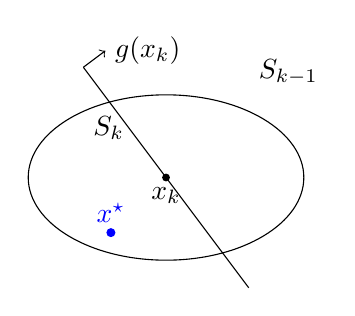
\begin{tikzpicture}[scale=0.7]
      \node (z0) at (0, 0) {};
      \node[draw=blue, inner sep=1, fill=blue, circle] (zstar) at (-1, -1) {};
      \node[above] at (zstar) {{\color{blue}$x^\star$}};
      \draw[black, rotate around={0:(z0)}] (z0) ellipse ({2.5} and {1.5});
      \node[above right=3em, black] at (z0) {$S_{k-1}$};

      \uncover<2->{
        \node[black, inner sep=1, fill, circle] at (z0) {};
        \node[below, black] at (z0) {$x_k$};
      }
      \uncover<3->{
        \draw[black] (-1.5, 2) -- (1.5, -2);
        \draw[->] (-1.5, 2) -- +($0.2*(2, 1.5)$) ;
        \node[right] at ($(-1.5, 2)+0.2*(2, 1.5)$) {$g(x_k)$};
        
        \node[above right=3em, black] at (-3, -1) {$S_k$};
      }

    \end{tikzpicture}
  \end{center}

  
  \begin{algorithm}[H]
    \SetKwInput{Initialization}{Initialisation}
    \Initialization{$S_0\defn Q$}
    \For{$k \in [1, 2, \dots]$}{
      Choose $x_k \in \interior(S_{k-1})$\\
      Call gradient oracle $g(x_k)\in \partial f(x_k)$\\
      Add cut
      \[
        S_k = S_{k-1} \cap \set{y}{\iprod{g(x_k)}{y-x_k}\leq 0}.
      \]
    }
    \caption{Cutting-Plane}
  \end{algorithm}

\end{frame}

\begin{frame}{Center of Gravity}

  \textbf{Definition:} The center of gravity of a set $S$ is defined as
  \[
    {\rm{cg}(S)}\defn \frac{\int_{S} x \d x}{\int_{S}\d x}.
  \]

  \vfill

  \textbf{Fact:} (Pie Cutting Theorem). Let $g$ be any vector. Define the set
  \[
    S_+ = S \cap \set{y}{\iprod{g}{y-\rm{cg}(S)}\leq 0}.
  \]
  Then,
  \[
    \frac{\int_{S_+}\d x}{\int_{S}\d x}\leq 1-\tfrac 1e.
  \]
\end{frame}

\begin{frame}{Cutting Plane Method}

  \textbf{Theorem:} (Nesterov) If $f$ is Lipschitz continuous and $\norm{x_0-x^\star}\leq D$, then cutting plane through center of gravity iterates
  satisfy
  \[
    f(x_N) - f^\star \leq L D (1-\tfrac 1e)^{\tfrac N n}.
  \]

  \vfill

  \textbf{Theorem:} (Nesterov) There exists a resisting oracle $\tilde f$ such that after $N$ oracle calls we have 
  \[
    \tilde f(x_N) - \tilde f^\star \geq L D (1/8)^{\tfrac N n}.
  \]
  

\end{frame}

\begin{frame}{Cutting Plane Method}

  \textbf{Remarks:}

  \begin{itemize}
  \item Bisection method is essentially optimal
  \item Complexity scales as $\mc O(n \log(LD/\epsilon))$
  \item<2-> Not practical!
  \end{itemize}

  
\end{frame}

\begin{frame}{Next week}

  Simple method for high-dimensional problems:
  \vfill
  \begin{center}
    \textbf{Subgradient Methods!}
  \end{center}
  
\end{frame}

\end{document}
%%% Local Variables:
%%% mode: latex
%%% TeX-master: t
%%% End:
